\documentclass[border=10pt]{standalone}
\usepackage{amsmath,amssymb}
\usepackage{pgfplots}
\pgfplotsset{compat=1.18}
\usetikzlibrary{arrows.meta}

\begin{document}
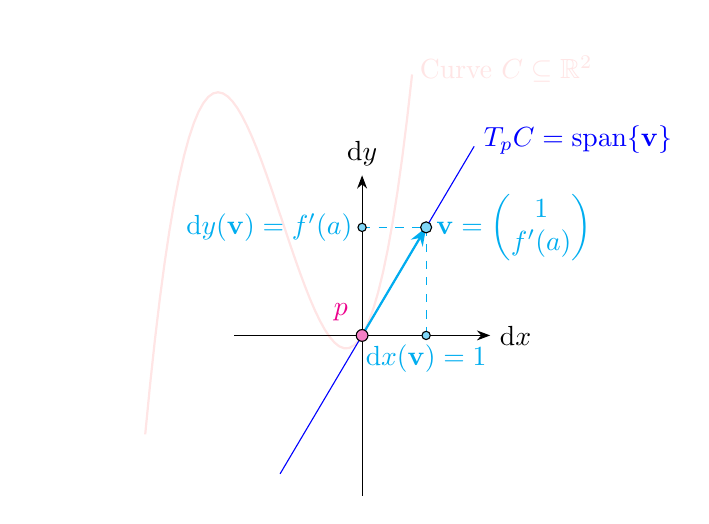
\begin{tikzpicture}
% --- Pre-calculate all values for the new function ---
\pgfmathsetmacro{\a}{2.25}              % x-coordinate of point p
\pgfmathsetmacro{\ay}{\a^3-3*\a^2+5} % y-coordinate using the new function
\pgfmathsetmacro{\slope}{3*\a^2 -6*\a} % Slope using the new derivative

\pgfmathsetmacro{\dx}{1}             % Vector x-component (made slightly smaller for visibility)
\pgfmathsetmacro{\dy}{\slope * \dx}   % Vector y-component
\pgfmathsetmacro{\endx}{\a + \dx}     % Vector end-point x
\pgfmathsetmacro{\endy}{\ay + \dy}     % Vector end-point y

% --- Pre-calculate label position for the tangent line ---
\pgfmathsetmacro{\labelx}{\a + 0.5}
\pgfmathsetmacro{\labely}{\ay + \slope*(\labelx-\a)}

\begin{axis}[
	axis lines=center,
	axis line style={opacity=0},
%	xlabel=$\mathrm{d}x$,ylabel=$\mathrm{d}y$,
	xtick=\empty,ytick=\empty,
	legend pos=north west,
	xmin=-2.5, xmax=5,   % Adjusted axis limits
	ymin=-1, ymax=6,    % Adjusted axis limits
	restrict y to domain=-1:6,
	axis equal, % Ensures slopes are visually correct
	clip=false,
	]
	
	\draw[-Stealth] (\a-2,\ay) to (\a+2,\ay) node[right] {$\mathrm{d}x$};
	\draw[-Stealth] (\a,\ay-2.5) to (\a,\ay+2.5) node[above] {$\mathrm{d}y$};
	
	% --- Plot the curve y = x^3 + x^2 + 1 ---
	\addplot[domain=-2.5:5, samples=100, thick, red, opacity=.1] {(x+1)*(x-2)*(x-2) + 1};
	\node[above right, red, opacity=.1] at (axis
	cs: 3, 3^3-3*3^2+5) {Curve $C\subseteq\mathbb{R}^2$};
	%	\draw[] (1,1) circle (2pt);
	% --- Plot the tangent line at x=a ---
	%	\addplot[domain=-1:3.5, samples=2, blue] {\ay + \slope*(x-\a)};
	%	\node[right, blue] at (axis cs:3.5, 3*3^2-13) {Tangent Space $T_pC$};
	
	% --- Draw the tangent vector v ---
	\addplot[domain=-2:4, samples=100, blue] {\ay + \slope*(x-\a)};
	\node[right, blue] at (axis cs:4, 4.25) {$T_pC=\mathrm{span}\{\mathbf{v}\}$};
	\draw[
	-{Stealth},
	thick,
	cyan,
	] (axis cs: \a, \ay) -- (axis cs: \endx, \endy)
	node[right] {$\mathbf{v}=\begin{pmatrix} 1\\ f'(a) \end{pmatrix}$};
	
%	\draw[-Stealth,red] (\a,\ay) to (\a+1,\ay);
%	\draw[-Stealth,red] (\a,\ay) to (\a,\ay+1);
	\draw[dashed, cyan] (\a,\ay+\slope) node[left] {$\mathrm{d}y(\mathbf{v})=f'(a)$} to (\a+1,\ay+\slope);
	\draw[dashed, cyan] (\a+\dx,\ay+\slope) to (\a+1,\ay) node[below] {$\mathrm{d}x(\mathbf{v})=1$};
	\draw[fill=cyan!50] (\a+\dx, \ay+\slope) circle (2pt);
	\draw[fill=cyan!50] (\a+\dx, \ay) circle (1.5pt);
	\draw[fill=cyan!50] (\a,\ay+\slope) circle (1.5pt);	
	
	% --- Mark the point p ---
	%	\draw[fill=magenta] (\a,\ay) circle (2pt) node[above, magenta] {$p$};
	%	\draw[dashed, magenta] (\a,\ay) to (\a,0) node[below] {$a$};
	%	\draw[dashed, magenta] (\a,\ay) to (0,\ay) node[left] {$f(a)$};
	\node[circle, fill=magenta!50, draw=black, inner sep=1.5pt, label={above left:$\color{magenta}p$}] at (axis cs: \a, \ay) {};
	%	\draw[fill=magenta!50] (\a,0) circle (1.5pt);
	%	\draw[fill=magenta!50] (0,\ay) circle (1.5pt);
\end{axis}
\end{tikzpicture}
\end{document}